\documentclass[12ptnotitlepage]{article}
\pagestyle{empty}

\usepackage[margin=2pt,papersize={7in, 9.6in}]{geometry}

\usepackage{mathtools}
\newcommand*{\pluseq}{\mathrel{{+}{=}}}
\usepackage{tikz}
\usetikzlibrary{arrows.meta,calc,fit,positioning,chains}
\definecolor{l3-color}{cmyk}{0,0.06,0.12,0}
\definecolor{l2-color}{cmyk}{0,0.2,0.4,0}
\definecolor{l1-color}{cmyk}{0,0.45,0.55,0}
\definecolor{reg-color}{cmyk}{0.15,0.8,0.8,0}

\tikzset{bpack/.style={to path={
      foreach \i in {1,...,#1} { -- ++(0.5, 0) -- ++ (-0.5,-0.4) } -- (\tikztotarget) \tikztonodes
    }},
  bpack/.default=6,
  apack/.style={to path={
      foreach \i in {1,...,#1} { -- ++(0, -0.5) -- ++(0.4,0.5) } -- (\tikztotarget) \tikztonodes
    }},
  apack/.default=6}

\tikzset{
  label-brace/.style={to path={
      (\tikztostart) ++(#1) -- ++(#1)
      -- ($(\tikztotarget) + 2 *(#1)$) \tikztonodes
      -- +($-1 *(#1)$)
    }},
  brace below/.style={label-brace={0, -3pt}},
  brace above/.style={label-brace={0, 3pt}},
  brace right/.style={label-brace={3pt, 0}},
  brace left/.style={label-brace={-3pt, 0}}}

\tikzset{
  dim-label/.style={label distance=0pt,inner sep=0},
}

\tikzset{
  our-arrow/.style={-{Latex[length=8pt,width=4pt]}},
}

\tikzset{
  memory/.style={fill=white},
  l3/.style={fill=l3-color},
  l2/.style={fill=l2-color},
  l1/.style={fill=l1-color},
  regs/.style={fill=reg-color},
  legend/.style={on chain=labels, minimum height=1ex, minimum width=1em,
    draw, rectangle, outer sep=0, label={[label distance=3pt]right:{\small #1}}}
}

\tikzset{
  loop-label/.style={midway, draw, rectangle},
  square-mat/.style={rectangle,draw,fit={(0, 0) (3, -3)},inner sep=0},
  wide-mat/.style={rectangle,draw,fit={(0, 0) (3, -1)},inner sep=0},
  tall-mat/.style={rectangle,draw,fit={(0, 0) (1, -3)},inner sep=0}
}

\newcommand*{\bpackarr}[2][6]{\draw[our-arrow] ($(#2 - 0.75, -0.25)$) to[bpack=#1] ++($(0.5, -0.4 * #1)$);}
\newcommand*{\apackarr}[2][6]{\draw[our-arrow] ($(0.25, - #2 + 0.75)$) to[apack=#1] ++($(0.4 * #1, -0.5)$);}

\newcommand*{\bracelabel}[4]{\draw (#1) to[brace #3]%
  node[midway,label={[dim-label]#3:#4}] {} (#2);}

\newcommand*{\packlabel}[3]{\path (#1) -- (#2)%
  node[midway,label={#3:pack}] {};}

% [style] name width height N code-for-every
\newcommand*{\vgrids}[6][fill=white]{
  \foreach \x in {1, ..., #5} {
    \node[rectangle, draw, #1,fit={($(#3 * \x - #3, 0)$) ($(#3 * \x, -#4)$)}, inner sep=0] (#2\x) {};
    #6
  }
}
% [style] name width height N code-for-every
\newcommand*{\hgrids}[6][fill=white]{
  \foreach \y in {1, ..., #5} {
    \node[rectangle, draw, #1,fit={($(0, -\y * #4 + #4)$) ($(#3, -\y * #4)$)}, inner sep=0] (#2\y) {};
    #6
  }
}

% [first-style] style name width height N code-for-every
\newcommand*{\vgridscache}[7][memory]{
  \foreach \x in {1, ..., #6} {
    \ifnum\x=1%
    \node[rectangle, draw, #1 ,fit={($(#4 * \x - #4, 0)$) ($(#4 * \x, -#5)$)}, inner sep=0] (#3\x) {};
    \else
    \node[rectangle, draw, #2 ,fit={($(#4 * \x - #4, 0)$) ($(#4 * \x, -#5)$)}, inner sep=0] (#3\x) {};
    \fi
    #7
  }
}
% [first-style] style name width height N code-for-every
\newcommand*{\hgridscache}[7][memory]{
  \foreach \y in {1, ..., #6} {
    \ifnum\y=1%
    \node[rectangle, draw, #1,fit={($(0, -\y * #5 + #5)$) ($(#4, -\y * #5)$)}, inner sep=0] (#3\y) {};
    \else
    \node[rectangle, draw, #2,fit={($(0, -\y * #5 + #5)$) ($(#4, -\y * #5)$)}, inner sep=0] (#3\y) {};
    \fi
    #7
  }
}

\newcommand*{\pluseqnode}[1]{\node[at={(0, -1.5)}] (#1-plus) {\large $\pluseq$};}

% [style] N N - 1 offset-right
\newcommand*{\loopborder}[3][black]{\draw[rounded corners, color=#1]%
  (#2-loop.west) -| ($(#3-rect-west) + (-5pt, -5pt)$) coordinate (#2-rect-west)%
  -- ($(#3-rect-east) + (5pt, -5pt)$) coordinate (#2-rect-east)%
  |- (#2-loop.east);}


\begin{document}
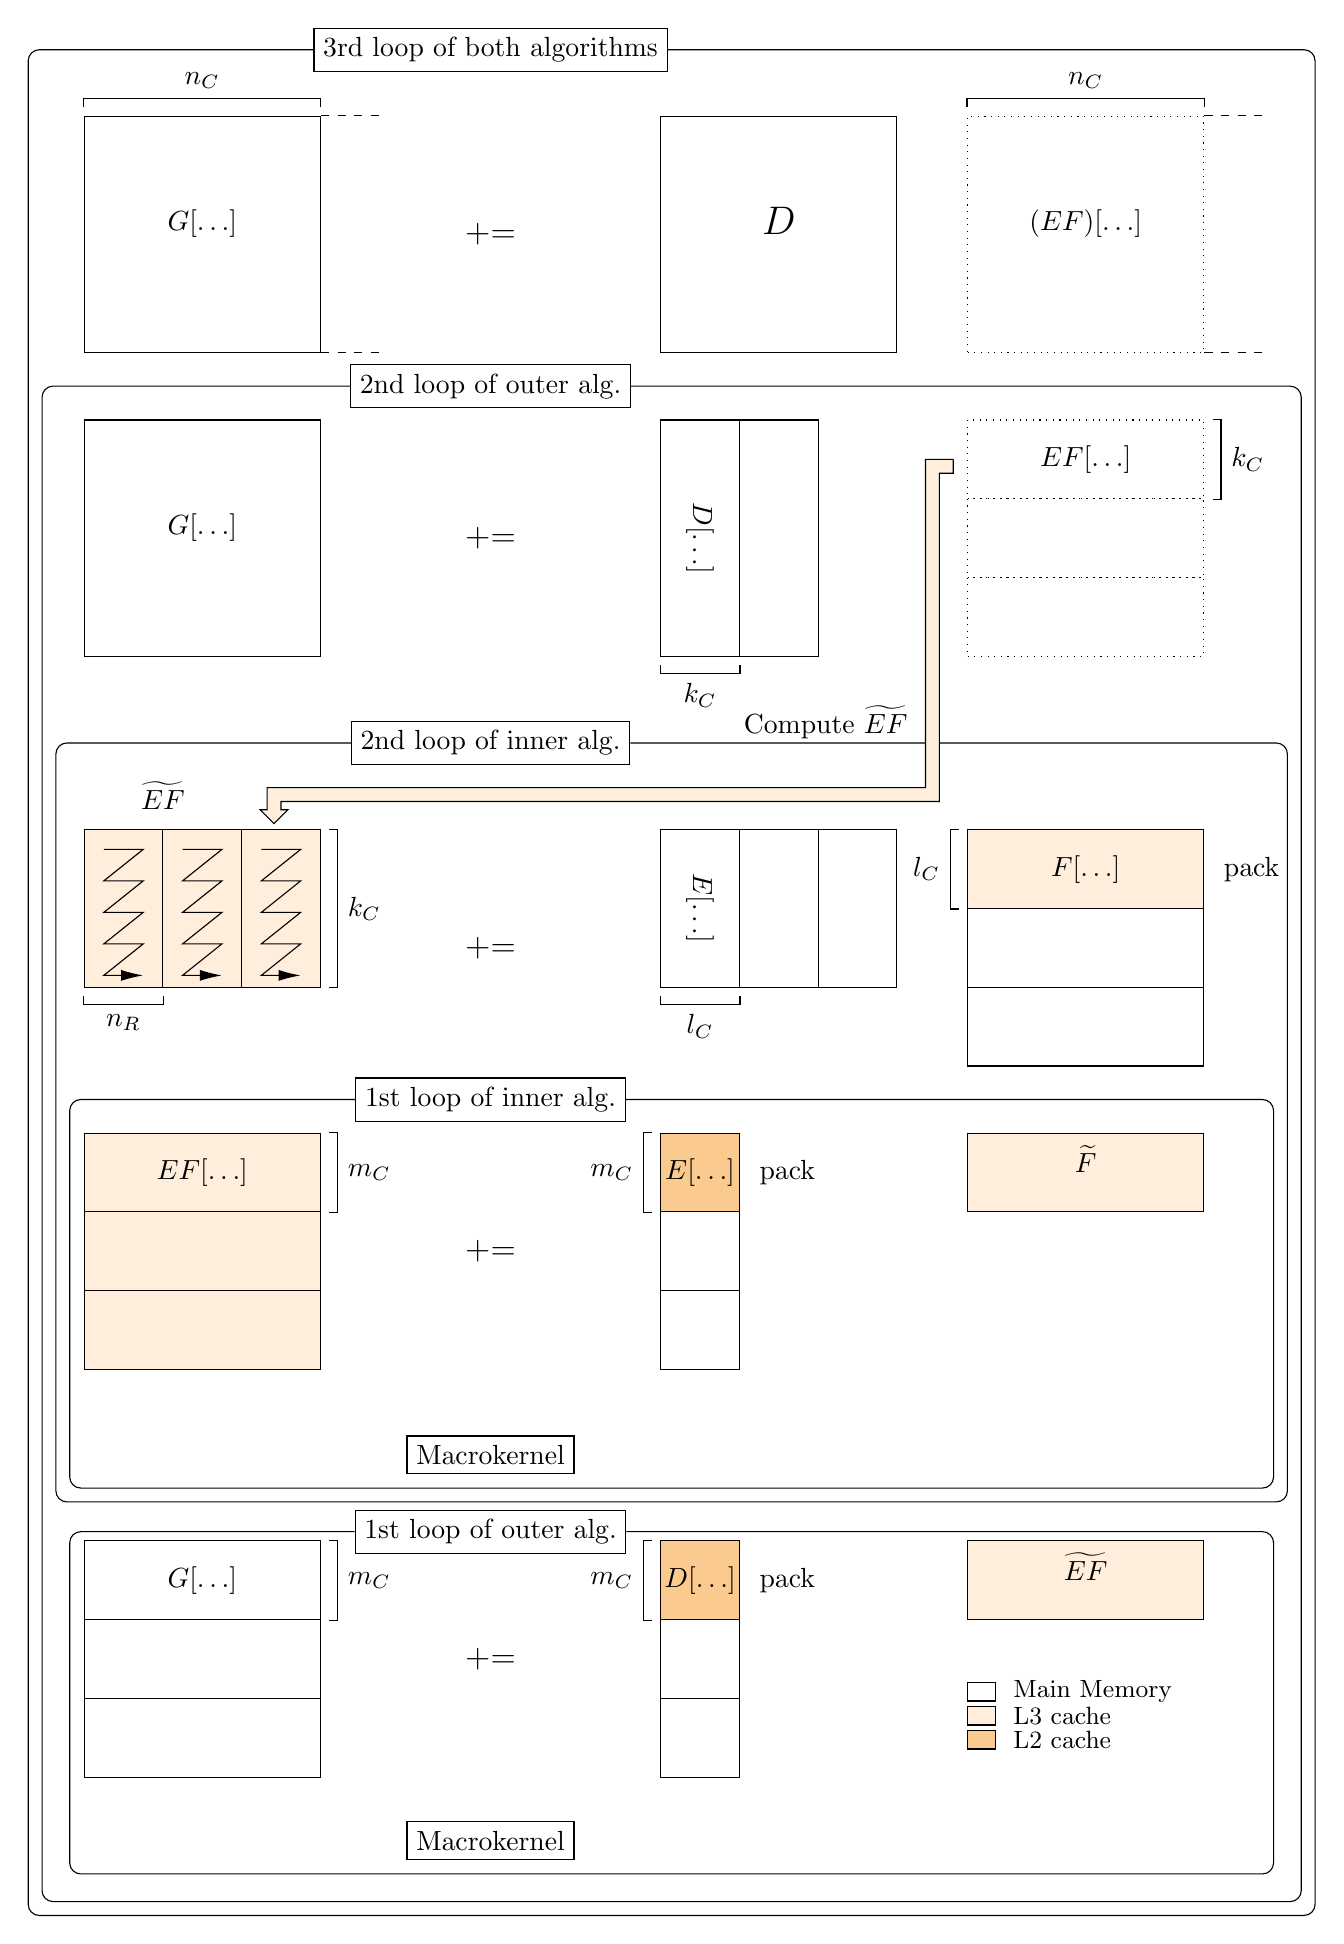
\begin{tikzpicture}
\matrix (loops)[column sep=0.2cm, row sep=5.5ex] {
  \node[square-mat] (3G) {$G[\ldots]$};
  \bracelabel{3G.north west}{3G.north east}{above}{$n_{C}$}
  \draw[dashed] (3G.north east) -- ++(0.75, 0)
  (3G.south east) -- ++(0.75, 0);&

  \pluseqnode{3o}&

  \node[square-mat,memory] (3D) {\Large $D$};&

  \node[square-mat,memory,dotted] (3EF) {$(EF)[\ldots]$};
  \bracelabel{3EF.north west}{3EF.north east}{above}{$n_{C}$}
  \draw[dashed] (3EF.north east) -- ++(0.75, 0)
  (3EF.south east) -- ++(0.75, 0);\\


  \node[square-mat,memory] (2G) {$G[\ldots]$};&

  \pluseqnode{2o}&

  \vgrids[memory]{2D}{1}{3}{2}{}
  \node[at=(2D1),rotate=-90] {$D[\ldots]$};
  \bracelabel{2D1.south west}{2D1.south east}{below}{$k_{C}$}&

  \hgrids[memory,dotted]{2EFo}{3}{1}{3}{}
  \node[at=(2EFo1)] {$EF[\ldots]$};
  \bracelabel{2EFo1.north east}{2EFo1.south east}{right}{$k_C$}\\

  %% Inner loop starts
  \vgrids[l3]{2EFi}{1}{2}{3}{\bpackarr[4]{\x}}
  \bracelabel{2EFi1.south west}{2EFi1.south east}{below}{$n_R$}
  \bracelabel{2EFi3.north east}{2EFi3.south east}{right}{$k_C$}
  \path (2EFi1.north west) -- (2EFi2.north east) node[midway,label={above:$\widetilde{EF}$}] {};&

  \pluseqnode{2i}&

  \vgrids[memory]{2E}{1}{2}{3}{}
  \node[at=(2E1),rotate=-90] {$E[\ldots]$};
  \bracelabel{2E1.south west}{2E1.south east}{below}{$l_C$}&

  \hgridscache[l3]{memory}{2F}{3}{1}{3}{}
  \node[at=(2F1)] {$F[\ldots]$};
  \bracelabel{2F1.north west}{2F1.south west}{left}{$l_C$}
  \packlabel{2F1.north east}{2F1.south east}{right}\\


  \hgrids[l3]{1EFi}{3}{1}{3}{}
  \node[at=(1EFi1)] {$EF[\ldots]$};
  \bracelabel{1EFi1.north east}{1EFi1.south east}{right}{$m_C$}&

  \pluseqnode{1i}&

  \hgridscache[l2]{memory}{1E}{1}{1}{3}{}
  \node[at=(1E1)] {$E[\ldots]$};
  \bracelabel{1E1.north west}{1E1.south west}{left}{$m_C$}
  \packlabel{1E1.north east}{1E1.south east}{right}&

  \node[wide-mat,l3] (1F) {$\widetilde{F}$};\\

  &\node[draw,rectangle] (kern-inner) {Macrokernel};&&\\

  %% Inner loop ends

  \hgrids[memory]{1G}{3}{1}{3}{}
  \node[at=(1G1)] {$G[\ldots]$};
  \bracelabel{1G1.north east}{1G1.south east}{right}{$m_C$}&

  \pluseqnode{1o}&

  \hgridscache[l2]{memory}{1D}{1}{1}{3}{}
  \node[at=(1D1)] {$D[\ldots]$};
  \bracelabel{1D1.north west}{1D1.south west}{left}{$m_C$}
  \packlabel{1D1.north east}{1D1.south east}{right}&

  \node[wide-mat,l3] (1EFo) {$\widetilde{EF}$};
  \begin{scoped}[start chain=labels going {below=2pt of \tikzchainprevious}]
    \node[legend=Main Memory, memory,anchor=north west] at (0, -1.8) {};
    \node[legend=L3 cache, l3] {};
    \node[legend=L2 cache, l2] (legend-anchor) {};
  \end{scoped}&\\
};
\path node[draw,above=1.8cm of 3o-plus] (3o-loop){3rd loop of both algorithms}
(3o-plus) -- (2o-plus) node[loop-label] (2o-loop){2nd loop of outer alg.}
(2o-plus) -- (2i-plus) node[loop-label] (2i-loop){2nd loop of inner alg.}
(2i-plus) -- (1i-plus) node[loop-label] (1i-loop){1st loop of inner alg.}
(kern-inner) -- (1o-plus) node[loop-label,pos=0.35] (1o-loop){1st loop of outer alg.}
node[draw, below=1.8cm of 1o-plus] (kern-outer) {Macrokernel};

\draw[rounded corners] let \p1 = ($(kern-outer.south) + (0pt, -5pt)$),
\p2 = ($(1EFo.south east) + (25pt, 0)$),
\p3 = ($(1G3.south west) + (-5pt, 0)$),
\p{east} = (\x2, \y1), \p{west} = (\x3, \y1) in
(1o-loop.west) -| (\p{west}) coordinate[below left=5pt and 5pt] (1o-rect-west)
-- (\p{east}) coordinate[below right=5pt and 5pt] (1o-rect-east)
|- (1o-loop.east);

\loopborder{2o}{1o}
\loopborder{3o}{2o}

\draw[rounded corners] let \p1 = ($(kern-inner.south) + (0pt, -5pt)$),
\p2 = ($(1F.south east) + (25pt, 0)$),
\p3 = ($(1EFi3.south west) + (-5pt, 0)$),
\p{east} = (\x2, \y1), \p{west} = (\x3, \y1) in
(1i-loop.west) -| (\p{west}) coordinate (1i-rect-west)
-- (\p{east}) coordinate (1i-rect-east)
|- (1i-loop.east);

\loopborder{2i}{1i}

\path[draw,l3] ($(2EFo1.west) + (-5pt, 0pt)$) -- ++(-10pt, 0pt) coordinate (inner-arr-start)
|- ($(2EFi3.north) + (-5pt, 15pt)$) node[pos=0.4,left=3pt] {Compute $\widetilde{EF}$} coordinate (inner-arr-down)
-- ++ (0pt, -8pt)
-- ++(-2.5pt, 0pt) -- ++(5pt, -5pt) -- ++(5pt, 5pt) -- ++(-2.5pt, 0pt)
-- ++ (0pt, 3pt)
-| ($(inner-arr-start) + (5pt, -5pt)$) -- ++(5pt, 0pt) -- ++(0pt, 5pt);
\end{tikzpicture}
\end{document}
